\documentclass[12pt,a4]{article}
% \usepackage{draftwatermark}
\usepackage{color}\usepackage{pdfpages}
\usepackage{background}
\usepackage{color}   %May be necessary if you want to color links
\usepackage{hyperref}
\hypersetup{
    colorlinks=true, %set true if you want colored links
    linktoc=all,     %set to all if you want both sections and subsections linked
    linkcolor=blue,  %choose some color if you want links to stand out
}
\textwidth 170 mm
\oddsidemargin -8 mm
\evensidemargin -8 mm
%\SetWatermarkScale{3.0}
\SetBgColor{red}
\SetBgOpacity{0.1}
\SetBgScale{10}

%\SetBgContents{\hspace{9mm}DRAFT \hspace{0mm}\vspace{2mm} 
\includegraphics[width=5mm]{Alfresco_logo_CMYK_white}} 
%\SetBgContents{\hspace{9mm} \hspace{0mm}\vspace{2mm} 
\includegraphics[width=5mm]{Alfresco_logo_CMYK_white}} 




\begin{document}
\begin{center}
{\huge Testing Alfresco using a python AJP client}

\vspace{5mm}


\vspace{25mm}

{\bf Alex Madon}

\vspace{5mm}

Alfresco Support

\vspace{5mm}

\today

\vspace{15mm}
% {\huge To be reviewed}

\end{center}
\vspace{5mm}

\newpage

\tableofcontents

\newpage

\section{Introduction}
AJP (Apache Jakarta Protocol) is a protocol often used to make a Apache proxy communicate with a Tomcat server.
The proxy can be for instance 
\begin{itemize}
\item an authentication layer, 
\item a load balancing layer 
\item or a SSL encryption layer.
\end{itemize}

Setting up a test environment to test or reproduce possible issue can be time consuming. You need to install the proxy software, launch the proxy daemon, configure the proxy.

The attached program is an AJP13 client that allows you to easily send AJP request for the command line, without having to install a full blown proxy. You can think that program as the 'curl' or AJP.


\section{Apache proxy}
Setting up an Apache proxy can be time consuming.
You will typically have to load several modules, e.g.
\begin{verbatim}
mod_auth_cas
mod_ssl
mod_proxy
\end{verbatim}

and declare the proxy mappings. below is a sample httpd.conf showing how to load the modules and the instructions to connect to the Alfresco back-ends.


\begin{verbatim}
LoadModule proxy_module modules/mod_proxy.so
LoadModule proxy_connect_module modules/mod_proxy_connect.so
LoadModule proxy_ajp_module modules/mod_proxy_ajp.so

<VirtualHost proxyajp.foo:80>
ServerName proxyajp.foo
ProxyRequests Off
ProxyPreserveHost On

ProxyPass /alfresco ajp://localhost:8009/alfresco
ProxyPassReverse /alfresco ajp://localhost:8009/alfresco
ProxyPassReverseCookiePath /alfresco /alfresco

ProxyPass /share ajp://localhost:8009/share
ProxyPassReverse /share ajp://localhost:8009/share
ProxyPassReverseCookiePath /share /share
</VirtualHost>
\end{verbatim}


\section{The AJP protocol}
The AJPv13 is described at:

\url{http://tomcat.apache.org/connectors-doc-archive/jk2/common/AJPv13.html}

It is a binary protocol. The main idea is to avoid few of the drawback of the stream oriented protocol that HTTP is by always sending packets for which you known in advance the length.
The same idea is used over and over again, and to send a string, you typically send the length of that string as an integer encoded on two bytes. That allows server programs to consume data, reading of the socket first the length of the data, then the data itself without having to parse the data to know where it ends, the data length being known in advance.
On the contrary to for instance parsing HTTP headers, where you do not know the length of the header and need to parse the header stream and look for the end of line characters (CR+LF, '\textbackslash r\textbackslash n', 0x0D0A)\cite{newline}



\section{Protocol analysis with wireshark}
It is useful to note that wireshark understands and decodes the AJPv13 protocol. The attached screen shot \ref{sc1}, shows how wireshark decodes AJP packets generated by our program.

\begin{figure}[htb]
\begin{center}
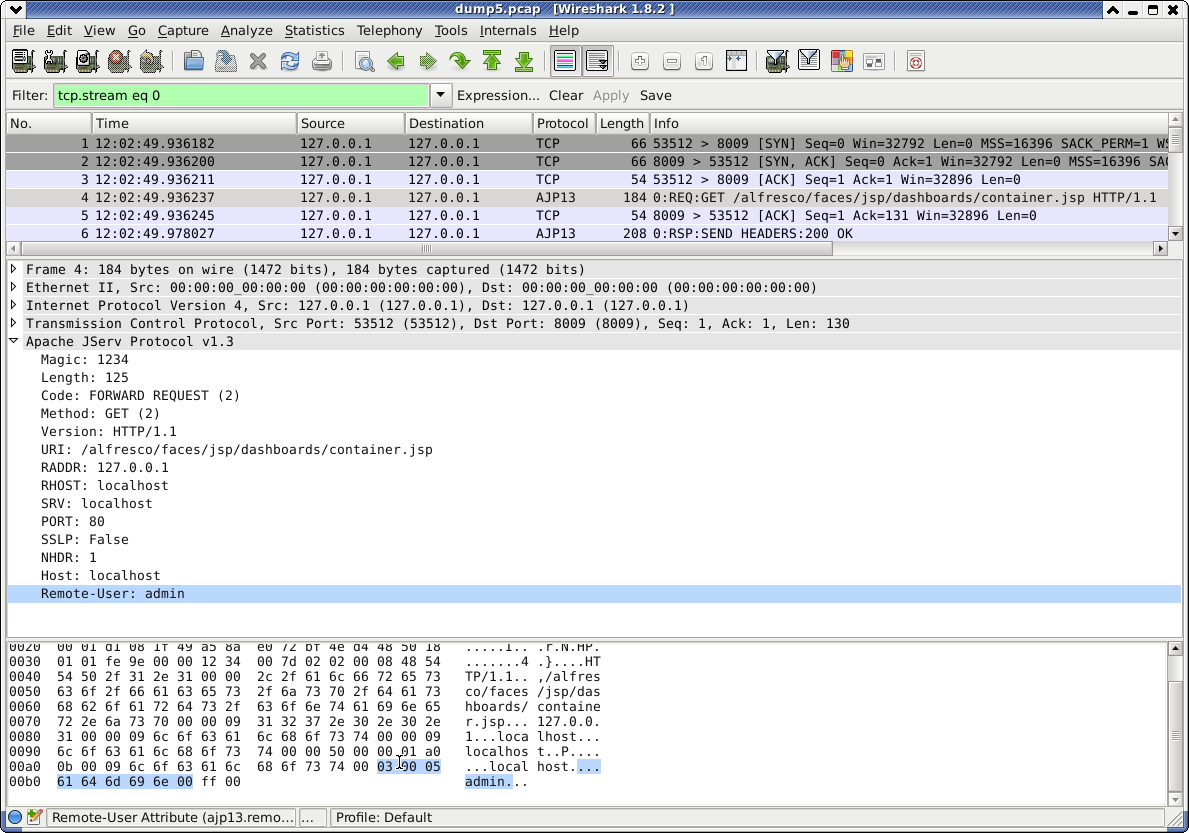
\includegraphics[width=180mm]{get_forward}
\caption{AJP packet decoding with wireshark.}
\label{sc1}
\end{center}
\end{figure}


\section{AJP implementations}

The most used AJP client is probably the Apache module mod\_ajp.
The module is written in C.
The server side AJP code most used is surely the Tomcat code.

Before writing our tool, we looked at available implementations on the Internet. Very few could be found apart the Apache C client and Java server code. Some tools were implemented the CPING AJP command, to be used in particular within monitoring tools like nagios\cite{nagios}
The C client code was not particularly adapted to a Support environment, where easy installation, portability and ease of change are important
An erlang implementation\cite{ajperlang} of the CPING and GET Request Forward helped us to grasp the logic of the protocol.


\section{Our implementation}

Our program is a python implementation of the protocol. Currently we implement the ``GET Forward Request'' and few other methods that are read only (no PUT, POST or DELETE).

You will need python version greater than 3.2.

\section{Getting the code}
The code and the documentation is available from the Support SVN repository\cite{svn} at:

\url{https://svn.alfresco.com/repos/support/ajpclient/}


\section{Program usage syntax}
The program is a command line tool. Its usage can be obtained using the -h option:

\begin{verbatim}
usage: ajprequest.py [-h] [-H HEADER] [-r REMOTE_USER] [-l {INFO,DEBUG}]
                     requesturl [passurl]

A python AJP client

positional arguments:
  requesturl            The request to the proxy front end, e.g. http://localh
                        ost/alfresco/faces/jsp/dashboards/container.jsp
  passurl               The proxy pass url (default:
                        ajp://localhost:8009/alfresco)

optional arguments:
  -h, --help            show this help message and exit
  -H HEADER, --header HEADER
                        adds a header
  -r REMOTE_USER, --remote_user REMOTE_USER
                        Sets the remote_user CGI variable
  -l {INFO,DEBUG}, --log_level {INFO,DEBUG}
                        Sets the log level. Logs are sent to STDERR.

The AJPv13 protocol is documented at: http://tomcat.apache.org/connectors-doc-
archive/jk2/common/AJPv13.html
\end{verbatim}

Note that the content of the body is sent to STDOUT and that DEBUG and INFO lines are sent to STDIN.
You can thus use verbose log levels, and still easily keep the data separately using redirects. For instance:

\begin{verbatim}
./ajprequest.py -r admin -l DEBUG https://localhost/alfresco/faces/jsp/dashboards/container.jsp > out.html
\end{verbatim}
will show on the STDOUT (the shell) the debug information, and the content of the page will be saved to a file ``out.html''.

\section{Usage examples}

\subsection{Testing external authentication}

To test external authentication, you could edit your server.xml tomcat file and set the tomcatAuthentication="false" on the AJP connector, i.e replace

\begin{verbatim}
<Connector port="8009" protocol="AJP/1.3" redirectPort="8443"/>
\end{verbatim}

\begin{verbatim}
<Connector port="8009" protocol="AJP/1.3" redirectPort="8443" tomcatAuthentication="false"/>
\end{verbatim}

and then use the ``-r'' option to set the REMOTE\_USER CGI variable.


Depending on what you need to see, you can use requests like those:
\begin{verbatim}
./ajprequest.py -r admin -l INFO https://localhost/alfresco/faces/jsp/dashboards/container.jsp 
./ajprequest.py -r admin -l INFO https://localhost/alfresco/faces/jsp/dashboards/container.jsp | grep --color admin
./ajprequest.py -r admin -l INFO https://localhost/alfresco/faces/jsp/dashboards/container.jsp > out.html
./ajprequest.py -r admin -l DEBUG https://localhost/alfresco/faces/jsp/dashboards/container.jsp > out.html
\end{verbatim}
The first one will output the INFO log lines and the content to the shell.
The second one will show the ``logged as'' information in HTML that show what is use is logged (i.e confirming external authentication works). The third and fourth lines will save the content to a file for further analysis and will show the log lines in the shell.


\subsection{Testing redirects}

Redirects are done using HTTP ``Location:'' headers, and this can be observed at the default log level:

\begin{verbatim}
./ajprequest.py -r admin https://localhost/alfresco
> GET https://localhost/alfresco (via ajp://localhost:8009/alfresco )
> remote_user: admin
< 302 Moved Temporarily
< Location https://localhost/alfresco/
\end{verbatim}


\subsection{Checking that cookies are set with the correct security level}

The AJP Alfresco server should understand that the cookies need to have the security level that corresponds to the request scheme used. That is if the request hitting the proxy is using HTTP, the the secure cookie flag should be false. If the request hitting the proxy is sent using HTTPS, then the secure cookie flag should be set to True:

\begin{verbatim}
 ./ajprequest.py -r admin http://localhost/alfresco/
> GET http://localhost/alfresco/ (via ajp://localhost:8009/alfresco )
> remote_user: admin
< 302 Moved Temporarily
< Set-Cookie JSESSIONID=3C4E93238C1EED19853AC7F36CB5E7D3; Path=/alfresco
< Location http://localhost/alfresco/faces/jsp/dashboards/container.jsp
< Content-Type text/html
< Content-Length 0
\end{verbatim}


\begin{verbatim}
./ajprequest.py -r admin https://localhost/alfresco/
> GET https://localhost/alfresco/ (via ajp://localhost:8009/alfresco )
> remote_user: admin
< 302 Moved Temporarily
< Set-Cookie JSESSIONID=6055261F29835C4A53D87E5A09E9DBD1; Path=/alfresco; Secure
< Location https://localhost/alfresco/faces/jsp/dashboards/container.jsp
< Content-Type text/html
< Content-Length 0
\end{verbatim}

\subsection{Showing values of CGI variables}
The AJPv13 specifications\cite{ajpv13} defines several variables that can transmitted to the AJP back-ends from the proxy. Those are mapped to servlet CGI variables. This can be seen using a small JSP script:


Just create a file 'test.jsp' at the location:

\begin{verbatim}
tomcat/webapps/alfresco/test.jsp
\end{verbatim}

and add the following content to it:


\begin{verbatim}
getRemoteUser: <% out.print(request.getRemoteUser()); %>
getAuthType: <% out.print(request.getAuthType() ); %>
getProtocol: <% out.print(request.getProtocol() ); %>
getScheme: <% out.print(request.getScheme() ); %>
getServerName: <% out.print(request.getServerName() ); %>
getServerPort: <% out.print(request.getServerPort() ); %>
getRemoteAddr: <% out.print(request.getRemoteAddr() ); %>
getRemoteHost: <% out.print(request.getRemoteHost() ); %>
getRemotePort: <% out.print (request.getRemotePort() ); %>
isSecure: <% out.print(request.isSecure() ); %>
\end{verbatim}

You can add any of the servlet methods defined in the servlet documentation\cite{httpservlet} \cite{servlet}.

Below is the output of calling the JSP script using our AJP client using two different front end URLs:

\begin{verbatim}
./ajprequest.py -r admin http://localhost/alfresco/test.jsp
> GET http://localhost/alfresco/test.jsp (via ajp://localhost:8009/alfresco )
> remote_user: admin
< 200 OK
< Set-Cookie JSESSIONID=EDC5988D174A4438E2BF4C8DFBE601EB; Path=/alfresco
< Content-Type text/html
< Content-Length 204
getRemoteUser: admin
getAuthType: null
getProtocol: HTTP/1.1
getScheme: http
getServerName: localhost
getServerPort: 80
getRemoteAddr: 127.0.0.1
getRemoteHost: 127.0.0.1
getRemotePort: 0
isSecure: false
\end{verbatim}

\begin{verbatim}
./ajprequest.py -r admin https://localhost/alfresco/test.jsp
> GET https://localhost/alfresco/test.jsp (via ajp://localhost:8009/alfresco )
> remote_user: admin
< 200 OK
< Set-Cookie JSESSIONID=3AC995BB7EF54780D9A9A3D020DE1ACE; Path=/alfresco; Secure
< Content-Type text/html
< Content-Length 205
getRemoteUser: admin
getAuthType: null
getProtocol: HTTP/1.1
getScheme: https
getServerName: localhost
getServerPort: 443
getRemoteAddr: 127.0.0.1
getRemoteHost: 127.0.0.1
getRemotePort: 0
isSecure: true
\end{verbatim}

The first example shows a call using HTTP, and the second using HTTPS. You can see how the servlet gets aware of the properties of the request that hits a proxy.


\section{Conclusion}
In this article we introduce a tool which is a pure python implementation of a subset of the AJPv13 protocol.
The tool is standalone and does not rely on external libraries. The tool can be used to quickly test how Alfresco behaves when receiving AJP Forward Requests. From a productivity point of view, it can be very interesting as it does not require the installation and configuration of an Apache proxy and its module (authentication, encryption, etc \dots)

\begin{thebibliography}{9}

\bibitem{nagios}
\url{http://www.nagios.org}

\bibitem{ajpv13}
\url{http://tomcat.apache.org/connectors-doc-archive/jk2/common/AJPv13.html}

\bibitem{ajperlang}
\url{http://easyerl.blogspot.co.uk/2007/07/erlang-and-jboss-talking-ajp13-part-i.html}

\bibitem{newline}
\url{http://en.wikipedia.org/wiki/Newline}


\bibitem{svn}
\url{https://svn.alfresco.com/repos/support/ajpclient/}

\bibitem{httpservlet}
\url{http://docs.oracle.com/javaee/6/api/javax/servlet/http/HttpServletRequest.html}

\bibitem{servlet}
\url{http://docs.oracle.com/javaee/6/api/javax/servlet/ServletRequest.html}

\end{thebibliography}


\end{document}
